\documentclass{standalone}
\usepackage[x11names, svgnames, rgb]{xcolor}
\usepackage[utf8]{inputenc}
\usepackage{tikz}
\usetikzlibrary{automata, positioning, arrows}
\usepackage{amsmath}

\begin{document}
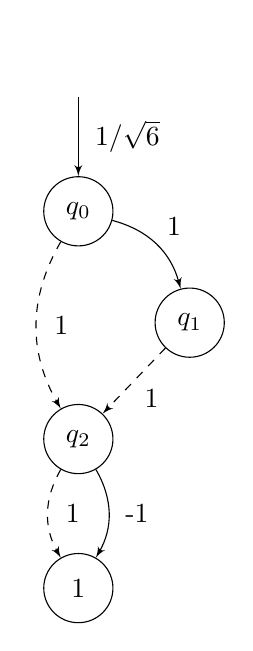
\begin{tikzpicture}[auto, every node/.style={shape=circle, align=center, solid, minimum size=0.01cm},>=latex']
  
  % Nodes definition
  \node[state] (q0) {$q_0$};
  \node[state] (q1) at ([shift={(-45:2cm)}]q0) {$q_1$};
  \node[state] (q2) [below = 2cm of q0] {$q_2$};
  \node[state] (1) [below = of q2] {1};
  \node[state, draw=none] (start) [above=of q0] {};

  % Edges definition
  \path[->]
  (start) edge node {$1/\sqrt{6}$} (q0)
  (q0) edge[bend right, dashed] node {1} (q2)
  (q0) edge[bend left] node {1} (q1)
  (q2) edge[bend right, dashed] node {1} (1)
  (q2) edge[bend left] node {-1} (1)
  (q1) edge[dashed] node {1} (q2);
  
\end{tikzpicture}
\end{document}
